% 09_iterations.tex
\chapter{Design iterations driven by verification}\label{sec:iterations}

The design space went through four iterations. None was planned: each was forced by a check on a result that the optimiser reported as a success. This chapter follows them in order, because each one added a rule to the design space that applies to any printed part optimised this way. \Cref{sec:optimisation_model} describes the model and the runs; \cref{sec:verification} the thresholded checks and the print geometry in full.

\begin{table}[htbp]
\centering\small
\caption{Design-space iterations: what each check found and what changed.}\label{tab:iter-summary}
\begin{tabularx}{\linewidth}{@{}lXX@{}}
\toprule
Result checked & Finding & Change for the next iteration, and rule\\
\midrule
Iteration 1 & structure meets every requirement at \SI{76.8}{g}, but no component can be installed & tub and lid; insertion, tool and cable paths as keep-outs\\
Iteration 2 & the receiver-antenna boss becomes a loose island & fixed antenna spine; every fixed region is kept by a load, a mass or a fixed link\\
Iteration 2, per part & a lid boss on the keel is held only by the lid; the GPS deck hangs from the lid & GPS deck moved to the tub, keel boss deleted; the rule applies within each part\\
Iteration 4 & GPS deck connected but carried by grey material; first mode \SI{146.8}{Hz} & keel zone cleaned, hand-drawn keels; connectivity is not stiffness\\
\bottomrule
\end{tabularx}
\end{table}

\section{Iteration 1: a structure that cannot be built}\label{sec:iter-1}

The first design space defined where every component sits: the battery plate as a fixed part of a one-piece centre body, voids above the flight controller for the receiver and the capacitor, a USB window, wire channels at the corners, a strap tunnel, and the rear keel under the GPS pad as design space. The production run on it converged to a feasible design after 28 cycles and was stopped after 40, with the frequency constraint and three of the four compliance caps active.

\subsection{The structure passed}

Thresholded at iso levels 0.5 and 0.3, both cuts met every requirement and were stiffer than the optimiser predicted (\cref{tab:iter-1}). The solid elements kept are fully stiff, while the optimiser counted grey ones at less than their share of the mass (\cref{tab:to-interp}), so grey material had not been over-credited. The design space was well separated: 47\,\% of the design elements below 0.3, 5\,\% between 0.3 and 0.5, and 48\,\% at or above 0.5. Cut at 0.4, smoothed and restored with the exact fixed regions, the frame weighed \SI{76.8}{g}: a body of \SI{45.58}{g} and four arms of \SI{7.81}{g}.

\begin{table}[htbp]
\centering\small
\caption{First design space, last cycle: optimiser against the thresholded bodies.}\label{tab:iter-1}
\begin{tabular}{@{}lrrr@{}}
\toprule
Model & First elastic mode & Modes 8 to 12 (Hz) & Compliance / cap\\
\midrule
Optimiser (grey) & \SI{417.8}{Hz} & 419.7 to 521.2 & 0.98 to 1.00\\
Thresholded, iso 0.5 & \SI{438.3}{Hz} & 446.1 to 547.4 & 0.86 to 0.93\\
Thresholded, iso 0.3 & \SI{449.5}{Hz} & 462.5 to 574.9 & 0.76 to 0.84\\
\bottomrule
\end{tabular}
\end{table}

\subsection{A check that stopped the wrong runs}

The runs on this design space also corrected a check. Spurious local modes (\cref{sec:to-spurious}) were guarded against by a rule that flagged any mode whose largest motion sat mostly in elements below density 0.3. It stopped a coarse run at cycle 10 and would have stopped the production run at cycle 20. The flagged modes were the arm bending modes: smooth, with their maxima at the motor seats, frequencies continuous with the history, and peak regions of thousands of nodes at mean densities of 0.2 to 0.45. The rule detected grey material in a mode, which is where the optimiser had made thin walls at the arm tips, not a spurious mode. The thresholded model, which measures the printable part directly, passed. From then on the mode check was a reported diagnostic, and the thresholded model at the print level became the acceptance test.

\subsection{The assembly failed}

Looked at as a part to build, the result was useless. The flight-controller bay was closed on every side: the only openings were the USB window, the strap tunnel, \SI{4}{mm} lead passages at the foot of each wall and slits of 1 to \SI{3}{mm} at the wall corners, and the roof was the fixed battery plate over an optimised ceiling. The board could not enter from any side, because 607 to \SI{861}{mm^3} of design material blocked each direction. The screw holes of its bosses were blind, with no screwdriver line, and nothing passed the battery lead, the GPS cable or the antenna.

The cause was in the design space, not in the optimiser. The design space said where each component sits but not how it gets there, and the optimiser filled every path, as it should: material that helps the stiffness and costs nothing under the constraints is material it keeps.

\subsection{Iteration 2: tub, lid and assembly paths}

The second design space was drawn around an assembly sequence (\cref{sec:arch-designspace}). The centre body became an open tub with a removable lid carrying the battery plate and, at this stage, the GPS deck. Every component received an insertion path, a tool path and a cable path as keep-outs, each checked by a sweep in an automated clash test. The board received \SI{4}{mm} of clearance on every side, so the body grew to $46\times46$\,mm and the corners moved out by \SI{3}{mm}. Each component got a designed seat and a retainer, with no glue or tape.

The lid created a new question: how is it connected to the tub? A reference analysis on the solid design space answered it. Tied at its screw bosses alone, the lid let a plate mode carrying the battery fall to \SI{405.1}{Hz} and pulled an arm saddle mode to \SI{389.8}{Hz}, below the goal. Tied over its whole seat on the tub rim, the same modes moved to 449.7 to \SI{654.6}{Hz}. In every static load case the battery's inertia presses the lid onto the rim and the screws preload it, so full contact is the real state as long as the seat is flat. The model ties the lid over the whole seat, and the printed lid underside and tub rim carry a flatness requirement of \SI{0.1}{mm}, checked with a feeler gauge before assembly.

The production run on iteration 2, thresholded at 0.4 with the seat tied, passed with a first mode of \SI{426.8}{Hz}. With the lid held at the five screw bosses only, the same body failed at \SI{192.1}{Hz}, a GPS deck mode below even the \SI{290}{Hz} minimum. The design relies on the seat contact, which the flatness requirement protects.

\section{Iterations 2 to 4: islands}\label{sec:iter-islands}

\subsection{An island at the antenna mount}

In iteration 2 the receiver antenna was held by a TPU clip screwed to a small fixed boss under the rear keel. In the optimisation that boss touched only design material and carried no load and no mass, because the antenna's mass was lumped with the flight controller. Nothing required a load path to it, so the optimiser removed the keel material around it. Thresholded, the boss was a loose part of \SI{0.15}{g} with six rigid-body modes between 45 and \SI{200}{Hz} on near-empty material.

Iteration 3 routed the antenna cable through a fixed sleeve, \SI{1.5}{mm} thick, from the bay into the keel, ending in a pad under the keel with an insert boss for the holder and a locating hole for its peg; a fixed web continues the sleeve up the rear wall into a lid boss. The chain from antenna to lid boss is fixed throughout, so the mount cannot be cut loose, and the antenna, holder, screw and insert (\SI{2.24}{g}) now act as a point mass on the pad. The antenna itself became a straight T (its moulded junction cannot bend), hanging vertically under the cable exit so the coax enters the stem without a bend, routed through one bend of radius \SI{7}{mm}, more than the six cable diameters the connector maker recommends. The spine added \SI{1.54}{g} of fixed material and passed 35 geometric checks, among them \SI{5.32}{mm} from the antenna legs to the rear arms.

The finding became a design-space rule: every fixed region either touches other fixed material or carries a load, a tie or a mass that needs a solid path. It is checked at export and after every thresholding by an island check.

\subsection{An island held by the other part}

The rule was then applied part by part. A lid boss on the keel carried the tie to the lid, and in the assembled model the lid held it. Checked on the tub alone, the boss was an island of \SI{141.4}{mm^3}, \SI{3.78}{mm} from the main tub at iso 0.4 and joined only by a chain of single elements between 0.3 and 0.4; all tub material behind it had been removed. The optimiser had used the lid as the boss's support. The GPS deck, then part of the lid, also hung from the lid as a cantilever.

Iteration 4 moved the GPS deck, with its pocket rim and cap bosses, from the lid to the tub, on top of the keel. The lid now ends at the battery plate with a \SI{0.5}{mm} gap to the deck and no tie between them, and the keel boss was deleted: the lid is clamped by the four wall bosses. Each lid screw pad is joined to the plate frame by a fixed link \SI{4.5}{mm} wide, so the lid's fixed region is one cell. The GPS mass now needs a load path through the tub, and the lid no longer supports anything it does not own. The rule was restated per part: each fixed region is kept by a load, a mass or a fixed link within its own part. The seat area shrank from 625.98 to \SI{363.23}{mm^2} on the tub side, and the full-density mass fell by \SI{0.09}{g}.

\section{Iteration 4: connected, but grey}\label{sec:iter-grey}

The production run on the fourth design space reduced the design volume by 55.4\,\% in 28 cycles (\cref{sec:optimisation_model}). The island check passed for every part at iso 0.3 and 0.4: the four wall bosses, the GPS deck and the lid were all connected. The thresholded model failed anyway. Its first elastic mode was a GPS deck mode at \SI{146.8}{Hz}, and the landing compliance exceeded its cap by 20\,\%. In the optimisation the deck had been carried at \SI{461.7}{Hz} by a wide block of keel material with densities mostly below 0.15. Such material is penalised in stiffness but still contributes, and no threshold keeps it: thresholded at any level from 0.3 to 0.5, the deck hung from two thin straps at its front.

\subsection{Five supports on the same density field}

Five supports were tested on the saved density field of the last cycle without a new optimisation, by forcing elements solid or empty inside a defined shape (\cref{tab:iter-keels,fig:iter-keels}).

\begin{table}[htbp]
\centering\small
\caption{Supports for the GPS deck, each checked as a thresholded model on the density field of the production run.}\label{tab:iter-keels}
\begin{tabular}{@{}lcccc@{}}
\toprule
Support & Model mass & First elastic mode & LC3a compliance / cap & Result\\
\midrule
As optimised, iso 0.4 & \SI{281.3}{g} & \SI{146.8}{Hz} & 1.20 & fail\\
As optimised, iso 0.3 & & \SI{162.3}{Hz} & & fail\\
Local iso 0.15 in the keel & \SI{281.5}{g} & \SI{380.6}{Hz} & 0.99 & fail\\
Two full side webs forced solid & \SI{283.4}{g} & \SI{430.7}{Hz} & 0.93 & pass\\
Keel zone cleaned, web B only & \SI{281.1}{g} & \SI{7.8}{Hz} & 28.05 & fail\\
Keel zone cleaned, keels A & \SI{282.2}{g} & \SI{420.7}{Hz} & 0.95 & pass\\
Keel zone cleaned, keels A and web B & \SI{282.3}{g} & \SI{428.4}{Hz} & 0.94 & pass\\
\bottomrule
\end{tabular}
\end{table}

\begin{figure}[htbp]
\centering
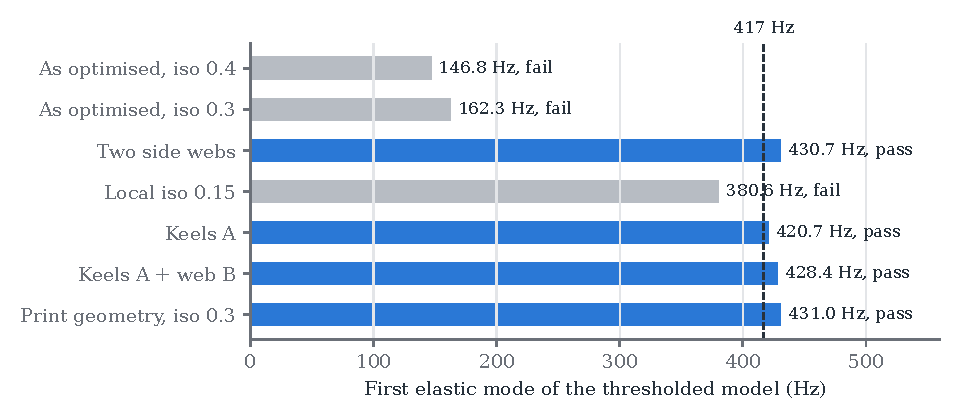
\includegraphics[width=0.95\linewidth]{plot_keels}
\caption{First elastic mode of each support variant against the \SI{417}{Hz} goal.}\label{fig:iter-keels}
\end{figure}

Lowering the threshold locally to 0.15 failed: the optimiser had not formed a structure in the keel at all, only a diffuse field. Two full-depth side webs passed, at \SI{2.11}{g} of forced material. The adopted design cleans the keel zone of all design material and adds two shapes drawn by hand, closer to what the optimiser had been building.
\begin{itemize}
\item \textbf{Keels A}: twin tapered keels hanging from the deck underside, mirrored in $y$, between $|y| = 4.6$ and the deck edge or the propeller sweep plus \SI{3}{mm}, flaring into the rear wall. Their depth grows towards the wall, where their bending moment is largest:
\begin{equation}
z_\text{bot}(x) = 21.5 - 11.5\left(0.6\,t + 0.4\,t^2\right), \qquad t = \frac{x + 50}{28},
\end{equation}
zero depth at $x = -50$ and \SI{11.5}{mm} deep at the wall.
\item \textbf{Web B}: a web \SI{2}{mm} thick under the antenna sleeve, from the sleeve to the rear wall, its lower edge one straight line from \SI{1}{mm} below the sleeve to the wall face at $z = -2.0$, \SI{1}{mm} above the opening for the motor leads.
\end{itemize}
Web B alone does not reach the deck and fails, but it braces the antenna spine: with it, mode 12 rises from 458.5 to \SI{529.6}{Hz}. Keels A and web B meet every requirement with \SI{1.1}{g} less than the side webs at the same margins, and the final print geometry with the exact solids reaches \SI{431.0}{Hz} (\cref{sec:verification}).

\begin{figure}[htbp]
\centering
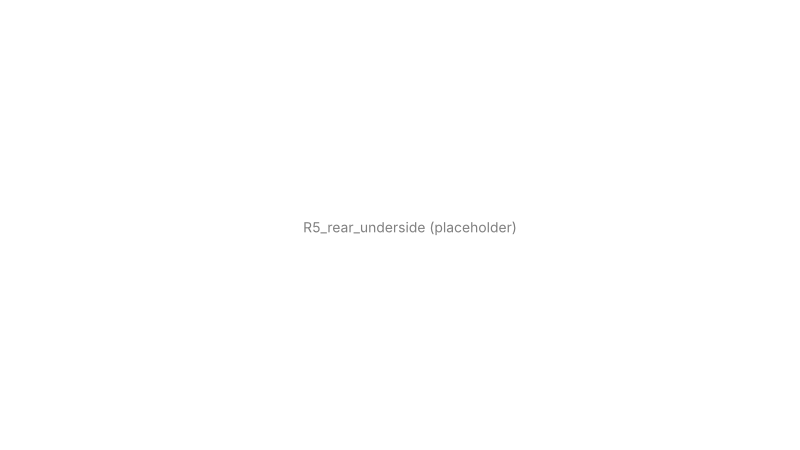
\includegraphics[width=0.85\linewidth]{R5_rear_underside}
\caption{Rear underside of the printed tub: twin keels under the GPS deck, the web under the antenna sleeve, the antenna pad and holder.}\label{fig:iter-rear}
\end{figure}

\subsection{Exact solids}

The keels were then drawn as exact solids for printing, from the same definitions (\cref{fig:iter-rear}). They differ from the element shapes of the check only where printability or mesh quality required it, and they hold more material, except for two pieces thinner than one element: each end stops with a face at least \SI{1}{mm} deep instead of a feather edge, every piece is at least \SI{1.2}{mm} wide, and the keels clip the cable channels and the propeller sweep exactly. Keels A are two solids of \SI{1315.1}{mm^3} (\SI{1.71}{g}) against \SI{1149.4}{mm^3} in the element shape, and web B is \SI{119.7}{mm^3} (\SI{0.16}{g}).

\section{Rules}\label{sec:iter-rules}

The four iterations left four rules, each stated so that it can be checked by a script.
\begin{enumerate}
\item \textbf{Assembly}: every component has an insertion path, a tool path and a cable path as keep-outs, checked by a sweep in the clash test.
\item \textbf{Connectivity}: every fixed region is kept by a load, a mass or a fixed link within its own part, checked at export and by an island check per part after every thresholding.
\item \textbf{Stiffness}: a fixed region that carries a mass or a load gets either a fixed load path to the main structure or a design corridor narrow enough that the optimiser must form a defined member in it. The thresholded model, not the island check, decides.
\item \textbf{Acceptance}: the result is accepted on the thresholded model at the print level, with every frequency and compliance requirement, not on the optimiser's grey model or on a mode diagnostic.
\end{enumerate}
The fourth design space would have revealed its grey keel within hours, not after a production run of seven and a half hours, if a coarse rehearsal had been thresholded and checked on its saved cycles first.
